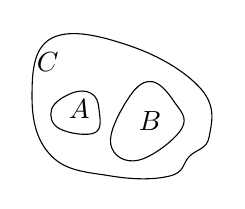
\begin{tikzpicture}[scale=0.5]
\draw  plot[smooth cycle, tension=.7] coordinates {(-5.5,3.8) (-7.5,4) (-8,2.5) (-7.5,1) (-6,0.5) (-4.5,0.5) (-4,1) (-3.5,1.5) (-3.7,2.7)};
\draw  plot[smooth cycle, tension=.7] coordinates {(-7.5,2.2) (-7.3,1.7) (-6.4,1.6) (-6.3,2.2) (-6.5,2.6) (-7,2.6) };
\draw  plot[smooth cycle, tension=.7] coordinates {(-6,1.3) (-5.3,0.9) (-4.2,1.7) (-4.4,2.4) (-5,2.9) (-5.6,2.4) };
\coordinate (C) at (-7.6,2.9) {} {};
\node[above] at (C) {$C$};
\coordinate (A) at (-6.8,1.7) {} {} {};
\node[above] at (A) {$A$};
\coordinate (B) at (-5,1.4) {} {} {};
\node[above] at (B) {$B$};
\end{tikzpicture}